LiveSync is based on the previous technique Remote Temporal Couplers (RTC) \cite{segundo2015remote} that intents to synchronize multiple contents related to the same main-content (MC). These contents may come from different Content Suppliers (CS), and range from video objects to extra content (EC), such as subtitles, additional information boards, labels, audio objects, or any other media artifacts that can me aligned over the same timeline.

RTC is based on three components: Main Content Provider, Content Suppliers, and User Devices (UD). Figure~\ref{rtc} \cite{segundo2015remote} shows the communication between these three components.

\begin{itemize}

\item \textit{MC Provider} is responsible for streaming the MC, that usually is a video stream transmitted over accessible channels to UD and CS.

\item \textit{Content Suppliers} provide EC related to a MC requested by UD. 

\item \textit{User Devices} are responsible to control one or more services provided by CS and playing the MC.
 
\end{itemize}


\begin{figure}[h!]
	\centering
	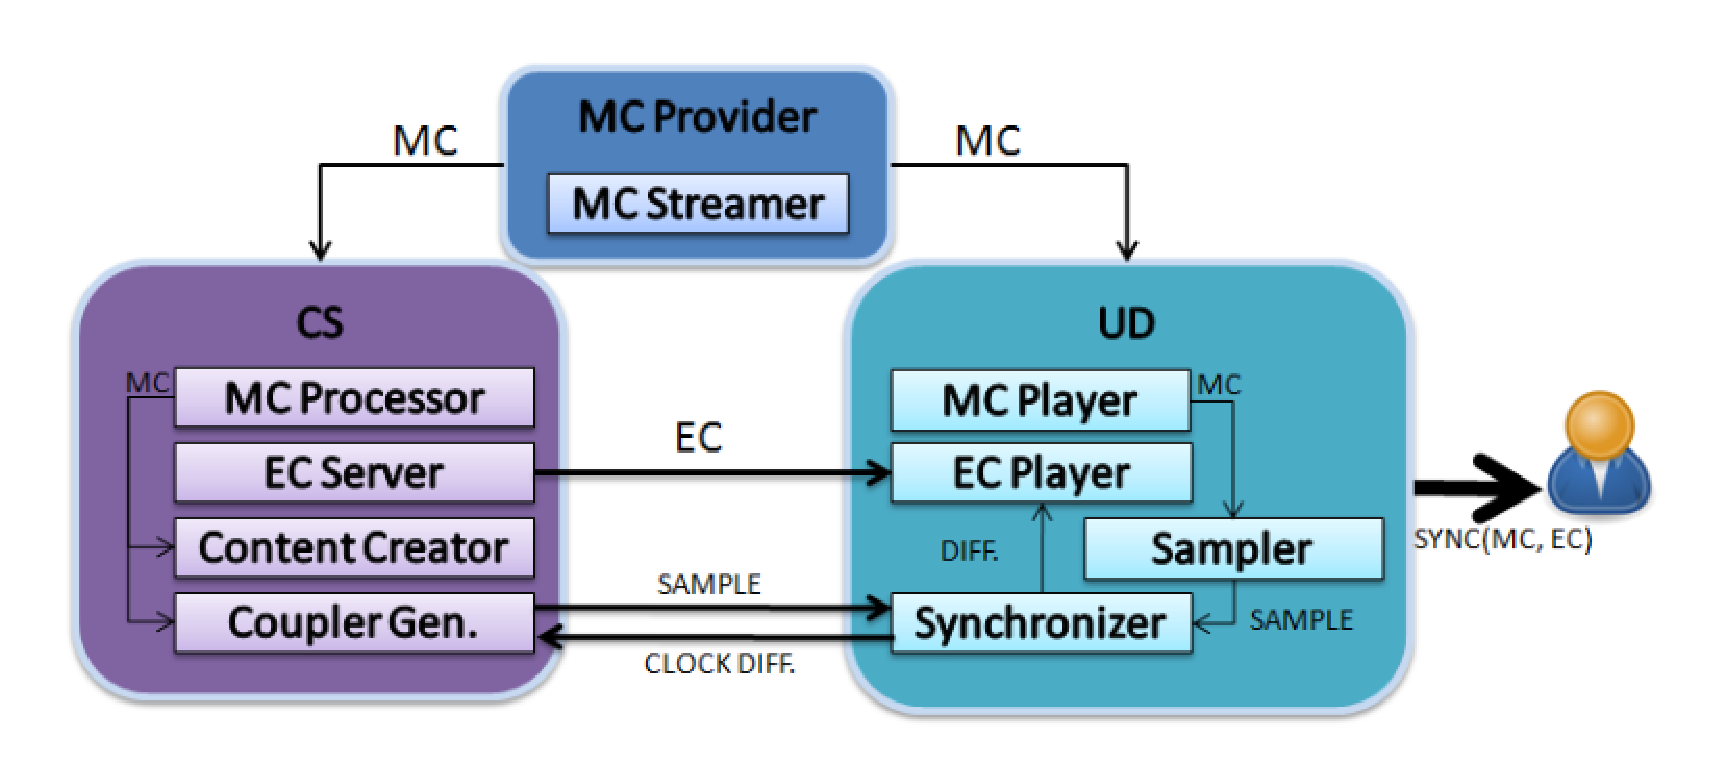
\includegraphics[scale=0.4]{figures/rtc}
	\caption{RTF - Entities Composition for Content Synchronization}
	\label{rtc}
\end{figure}

RTC consider that MC Providers usually offers no explicit timing information in its content to support the synchronization. Although, CS can provide synchronized content without depending on a explicit time specification sent by the MC Provider. The way found for reach synchronization into this scenario is delegate to CS the responsibility  for generate temporal couplers. A temporal coupler is an structure that relates a scene to the local timestamp, associated with it on a CS. In other words, for each scene $Sx$ presented by a CS, it provides a temporal coupler \textit{[Sx, Timestamp]} that identifies the local time when the scene occurred in its local timeline.

Finally, the RTC technique uses the timestamp into each temporal coupler to synchronize the contents from multiple Content Suppliers, as well to compose a coherent presentation in a mash-up application, in which users can choose what contents should be included.

Although LiveSync approach to synchronize video streams is based on RTC, it uses relational couplers, instead the temporal couplers used by RTC. A relational coupler relates pairs of videos and the $\Delta{time}$ between them. In this approach, alignment is constructed by relating a set of video streams, pair to pair, to generate coverage on the event timeline, rather than taking on a main-stream and to align each other stream with it. Moreover temporal couplers still are used in LiveSync to correctly play the synchronized streams.









